\documentclass[11pt,letterpaper]{article}
% Preamble for "The directed lattice two-neighbour graph percolates in every dimension"
\IfFileExists{lmodern.sty}{\usepackage[T1]{fontenc}\usepackage{lmodern}}{}
\usepackage[british]{babel}
\usepackage{amsmath,amsthm,amssymb,mathtools}
\usepackage[margin=1.05in]{geometry}
\usepackage{microtype}
\setlength{\emergencystretch}{1em}
\usepackage{xcolor}
\definecolor{paperlink}{RGB}{0,0,114}
\usepackage{tikz}
\usetikzlibrary{arrows.meta}
\definecolor{clusterblue}{RGB}{0,0,114}
\tikzset{
  v/.style={circle,fill=black!35,inner sep=0pt,minimum size=2.2pt},
  cv/.style={circle,fill=clusterblue,inner sep=0pt,minimum size=4.2pt},
  orig/.style={circle,draw=clusterblue,line width=0.9pt,inner sep=0pt,minimum size=8pt},
  entry/.style={rectangle,draw=clusterblue,line width=0.8pt,inner sep=0pt,minimum size=6pt},
  edge/.style={-{Stealth[length=2.6pt,width=2.2pt]},black!40,line width=0.45pt},
  clus/.style={-{Stealth[length=3.4pt,width=2.8pt]},clusterblue,line width=0.95pt},
  ign/.style={-{Stealth[length=3pt,width=2.6pt]},black!65,densely dashed,line width=0.6pt},
  explored/.style={black!8},
  guide/.style={black!55,line width=0.5pt},
}

\usepackage{booktabs}
\usepackage{hyperref}
\hypersetup{colorlinks=true,linktoc=all,
  linkcolor=paperlink,citecolor=paperlink,urlcolor=paperlink,pdfstartview=Fit,
  pdftitle={The directed lattice two-neighbour graph percolates in every dimension},
  pdfauthor={Benedikt Jahnel, Jonas K\"oppl}}
\usepackage[capitalise,nameinlink]{cleveref}
\crefname{figure}{Figure}{Figures}
\Crefname{figure}{Figure}{Figures}
\usepackage{enumitem}
\setlist[itemize]{leftmargin=2em,itemsep=0.25em,topsep=0.35em}
\setlist[enumerate]{leftmargin=2.25em,itemsep=0.25em,topsep=0.35em}
\setlength{\parindent}{1.25em}
\setlength{\parskip}{0pt}
\usepackage{fancyhdr}
\pagestyle{fancy}
\fancyhf{}
\fancyhead[L]{\small The directed lattice two-neighbour graph percolates in every dimension}
\fancyhead[R]{\small\thepage}
\setlength{\headheight}{14pt}
\numberwithin{equation}{section}

\usepackage{dsfont}
\newcommand{\1}{\mathds 1}

\theoremstyle{plain}
\newtheorem{theorem}{Theorem}[section]
\newtheorem{proposition}[theorem]{Proposition}
\newtheorem{lemma}[theorem]{Lemma}
\newtheorem{corollary}[theorem]{Corollary}
\theoremstyle{definition}
\newtheorem{definition}[theorem]{Definition}
\theoremstyle{remark}
\newtheorem{remark}[theorem]{Remark}

\newcommand{\Z}{\mathbb Z}
\newcommand{\N}{\mathbb N}
\renewcommand{\P}{\mathbb P}
\newcommand{\E}{\mathbb E}
\newcommand{\cD}{\mathcal D}
\newcommand{\cC}{\mathcal C}
\newcommand{\cG}{\mathcal G}
\newcommand{\cV}{\mathcal V}
\newcommand{\pc}{p_{\mathrm c}}
\newcommand{\kc}{k_{\mathrm c}}
\newcommand{\bond}{\mathrm{bond}}
\newcommand{\iid}{\mathrm{iid}}


\title{The directed lattice two-neighbour graph percolates in every dimension}
\author{Benedikt Jahnel\thanks{Institut f\"ur Mathematische Stochastik, Technische Universit\"at Braunschweig, Germany, and Weierstrass Institute for Applied Analysis and Stochastics, Berlin, Germany. \texttt{benedikt.jahnel@tu-braunschweig.de}. ORCID:~\mbox{\href{https://orcid.org/0000-0002-4212-0065}{0000-0002-4212-0065}}.} \and Jonas K\"oppl\thanks{Institut f\"ur Mathematische Stochastik, Universit\"at M\"unster, Germany. \texttt{jonas.koeppl@uni-muenster.de}. ORCID:~\mbox{\href{https://orcid.org/0000-0001-9188-1883}{0000-0001-9188-1883}}.}}
\date{}

\begin{document}
\maketitle
\thispagestyle{plain}

\begin{abstract}
In the directed $k$-neighbour graph on $\Z^d$, every vertex independently chooses $k$ of its $2d$ nearest neighbours uniformly at random and sends a directed edge to each of them. We prove that the directed $2$-neighbour graph percolates in every dimension $d\ge3$, with a lower bound on the percolation probability that does not depend on~$d$. Together with the planar case, this shows that the directed and the undirected $k$-neighbour graph on $\Z^d$ percolate if and only if $k\ge2$, in every dimension. The proof removes one coordinate at a time: all vertices of a vertical column jointly provide the out-edges of a single vertex in one dimension lower. For exchangeable local laws this projection acts on avoidance probabilities through an explicit monotone recursion, and an exact algebraic inequality between consecutive dimensions shows that the resulting bounds improve with~$d$. The argument ends in the plane with a local-to-global comparison principle and Kesten's theorem. The same recursion gives rigorous computer-assisted upper bounds on the critical mean out-degree, which we compare with simulations, and we discuss its monotonicity in the dimension.
\end{abstract}

\section{Introduction}\label{sec:intro}

Nearest-neighbour graphs are a basic model of spatial networks with a degree constraint. In the continuum, every point of a homogeneous Poisson point process is joined to its $k$ nearest neighbours, and the question is for which $k$ an infinite cluster exists \cite{HM96,BB13}. The lattice version, introduced in \cite{JKLT25}, keeps the degree constraint and replaces geometric distances by the nearest-neighbour structure of $\Z^d$: every vertex independently chooses $k$ of its $2d$ neighbours uniformly at random and sends a directed edge to each of them.

For $k=1$ this graph never percolates \cite{JKLT25}. For $k\ge d+1$ it percolates almost surely, by a simple monotone-path argument, and percolation was also shown for $k\ge4$ in $d\ge4$ and for $k=3$ in $d\ge5$ \cite{JKLT25}. The planar case $k=d=2$ was settled in \cite{CHJK26}, which also gives $k=d$ in every dimension \cite[Corollary~2.4]{CHJK26}, and a local-to-global comparison principle gave $k=3$ in $d=4$ and $k=2$ in all sufficiently large, but unspecified, dimensions \cite{BJKLRT25}. What remained open was $k=2$ in every specific dimension $d\ge3$. This case is not accessible to the second-moment method of \cite{CD83,JKLT25}: for $k=2$ the expected number of forward choices of a vertex equals one, so the expected number of open oriented paths of length $n$ from the origin equals one for every~$n$, as for a critical branching process.

We close this gap. The directed $2$-neighbour graph percolates in every dimension $d\ge3$ (\cref{thm:main}), and hence the directed and the undirected $k$-neighbour graphs percolate if and only if $k\ge2$, in all dimensions (\cref{cor:classification}). This confirms \cite[Conjecture~3.1]{JKLT25}. The proof is short and uses the extra dimensions directly. It is inspired by the coupling argument behind \cite[Theorem~2.3]{JKLT25}, which shows $\theta_d(k)\le\theta_{d+1}(k+1)$: there, the out-edges of a vertex of $\Z^d$ are produced by the vertices of the column above it in $\Z^{d+1}$, explored along vertical edges, and the out-cluster is explored column by column. Here, a vertex of $\Z^{d-1}$ is represented by an entire column of $\Z^d$, and the planar choices collected along the explored part of the column serve as its out-set. Iterating down to $\Z^2$ and tracking avoidance probabilities through an explicit recursion, we reach a planar model that dominates supercritical i.i.d.\ bond percolation in the sense of \cite{BJKLRT25}.

\cref{sec:setting} introduces the model and states the results, including rigorous upper bounds on the critical mean out-degree and a comparison with simulations. \cref{sec:discussion} discusses monotonicity in the dimension, the behaviour in high dimensions and further open problems. \cref{sec:proofs} contains the proofs.

\section{Setting and main results}\label{sec:setting}

For $d\in\N$ let $\cD_d\coloneqq\{\pm e_1,\dots,\pm e_d\}$ be the set of the $2d$ nearest-neighbour directions in $\Z^d$. A \emph{local law} is a probability measure $\mu$ on the subsets of $\cD_d$. The associated \emph{site-i.i.d.\ directed model} is the random directed graph on $\Z^d$ in which every vertex $x$ independently draws a set $N_x\subseteq\cD_d$ with law $\mu$ and sends a directed edge to every $x+u$ with $u\in N_x$. We write $\P_\mu$ for its law, $x\rightsquigarrow y$ if there is a directed path from $x$ to~$y$, $\cC(o)\coloneqq\{y\in\Z^d\colon o\rightsquigarrow y\}$ for the out-cluster of the origin~$o$, and
\begin{equation*}
\theta_d(\mu)\coloneqq\P_\mu\big(\#\cC(o)=\infty\big)\,.
\end{equation*}
With the $\ell^1$-ball $B_n\coloneqq\{x\in\Z^d\colon\|x\|_1\le n\}$ and $\partial B_n\coloneqq B_{n+1}\setminus B_n$, the \emph{one-arm probabilities} $\P_\mu(o\rightsquigarrow\partial B_n)$ decrease to $\theta_d(\mu)$ as $n\to\infty$. For $1\le k\le 2d$ let $\mu_{d,k}$ be the uniform distribution on the $k$-element subsets of $\cD_d$. The site-i.i.d.\ model with local law $\mu_{d,k}$ is the \emph{directed $k$-neighbour graph}, and we write $\theta_d(k)\coloneqq\theta_d(\mu_{d,k})$. Its \emph{undirected} version contains the undirected edge $\{x,y\}$ whenever at least one of the directed edges $(x,y)$, $(y,x)$ is present, and its \emph{bidirectional} version whenever both are present. \cref{fig:model} shows a sample in $d=2$. Finally, $\theta^\bond_d(p)$ denotes the probability that the origin lies in an infinite cluster of i.i.d.\ bond percolation on $\Z^d$ with parameter~$p$.

\begin{figure}[!htb]
\centering
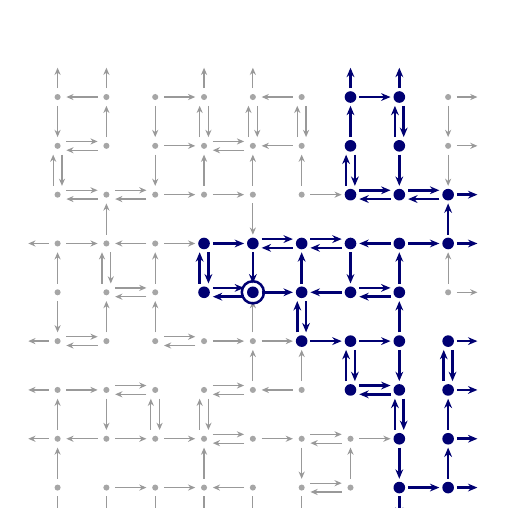
\begin{tikzpicture}[scale=0.62]
\draw[edge] (-4.00,-4.18) -- (-4.00,-4.60);
\draw[edge] (-4.00,-3.82) -- (-4.00,-3.18);
\draw[edge] (-4.00,-2.82) -- (-4.00,-2.18);
\draw[edge] (-4.18,-3.00) -- (-4.60,-3.00);
\draw[edge] (-4.18,-2.00) -- (-4.60,-2.00);
\draw[edge] (-3.82,-2.00) -- (-3.18,-2.00);
\draw[edge] (-3.82,-0.91) -- (-3.18,-0.91);
\draw[edge] (-4.18,-1.00) -- (-4.60,-1.00);
\draw[edge] (-4.00,-0.18) -- (-4.00,-0.82);
\draw[edge] (-4.00,0.18) -- (-4.00,0.82);
\draw[edge] (-3.82,1.00) -- (-3.18,1.00);
\draw[edge] (-4.18,1.00) -- (-4.60,1.00);
\draw[edge] (-3.82,2.09) -- (-3.18,2.09);
\draw[edge] (-4.09,2.18) -- (-4.09,2.82);
\draw[edge] (-3.91,2.82) -- (-3.91,2.18);
\draw[edge] (-3.82,3.09) -- (-3.18,3.09);
\draw[edge] (-4.00,3.82) -- (-4.00,3.18);
\draw[edge] (-4.00,4.18) -- (-4.00,4.60);
\draw[edge] (-3.00,-4.18) -- (-3.00,-4.60);
\draw[edge] (-2.82,-4.00) -- (-2.18,-4.00);
\draw[edge] (-3.18,-3.00) -- (-3.82,-3.00);
\draw[edge] (-2.82,-3.00) -- (-2.18,-3.00);
\draw[edge] (-2.82,-1.91) -- (-2.18,-1.91);
\draw[edge] (-3.00,-2.18) -- (-3.00,-2.82);
\draw[edge] (-3.18,-1.09) -- (-3.82,-1.09);
\draw[edge] (-3.00,-0.82) -- (-3.00,-0.18);
\draw[edge] (-2.82,0.09) -- (-2.18,0.09);
\draw[edge] (-3.09,0.18) -- (-3.09,0.82);
\draw[edge] (-2.91,0.82) -- (-2.91,0.18);
\draw[edge] (-3.00,1.18) -- (-3.00,1.82);
\draw[edge] (-2.82,2.09) -- (-2.18,2.09);
\draw[edge] (-3.18,1.91) -- (-3.82,1.91);
\draw[edge] (-3.18,2.91) -- (-3.82,2.91);
\draw[edge] (-3.00,3.18) -- (-3.00,3.82);
\draw[edge] (-3.18,4.00) -- (-3.82,4.00);
\draw[edge] (-3.00,4.18) -- (-3.00,4.60);
\draw[edge] (-2.00,-4.18) -- (-2.00,-4.60);
\draw[edge] (-1.82,-4.00) -- (-1.18,-4.00);
\draw[edge] (-2.09,-2.82) -- (-2.09,-2.18);
\draw[edge] (-1.82,-3.00) -- (-1.18,-3.00);
\draw[edge] (-1.91,-2.18) -- (-1.91,-2.82);
\draw[edge] (-2.18,-2.09) -- (-2.82,-2.09);
\draw[edge] (-2.00,-0.82) -- (-2.00,-0.18);
\draw[edge] (-1.82,-0.91) -- (-1.18,-0.91);
\draw[edge] (-2.18,-0.09) -- (-2.82,-0.09);
\draw[edge] (-2.00,0.18) -- (-2.00,0.82);
\draw[edge] (-1.82,1.00) -- (-1.18,1.00);
\draw[edge] (-2.18,1.00) -- (-2.82,1.00);
\draw[edge] (-1.82,2.00) -- (-1.18,2.00);
\draw[edge] (-2.18,1.91) -- (-2.82,1.91);
\draw[edge] (-2.00,2.82) -- (-2.00,2.18);
\draw[edge] (-1.82,3.00) -- (-1.18,3.00);
\draw[edge] (-1.82,4.00) -- (-1.18,4.00);
\draw[edge] (-2.00,3.82) -- (-2.00,3.18);
\draw[edge] (-1.00,-4.18) -- (-1.00,-4.60);
\draw[edge] (-1.00,-3.82) -- (-1.00,-3.18);
\draw[edge] (-0.82,-2.91) -- (-0.18,-2.91);
\draw[edge] (-1.09,-2.82) -- (-1.09,-2.18);
\draw[edge] (-0.82,-1.91) -- (-0.18,-1.91);
\draw[edge] (-0.91,-2.18) -- (-0.91,-2.82);
\draw[edge] (-1.18,-1.09) -- (-1.82,-1.09);
\draw[edge] (-0.82,-1.00) -- (-0.18,-1.00);
\draw[clus] (-1.09,0.18) -- (-1.09,0.82);
\draw[clus] (-0.82,0.09) -- (-0.18,0.09);
\draw[clus] (-0.82,1.00) -- (-0.18,1.00);
\draw[clus] (-0.91,0.82) -- (-0.91,0.18);
\draw[edge] (-0.82,2.00) -- (-0.18,2.00);
\draw[edge] (-1.00,2.18) -- (-1.00,2.82);
\draw[edge] (-0.82,3.09) -- (-0.18,3.09);
\draw[edge] (-1.09,3.18) -- (-1.09,3.82);
\draw[edge] (-0.91,3.82) -- (-0.91,3.18);
\draw[edge] (-1.00,4.18) -- (-1.00,4.60);
\draw[edge] (-0.18,-4.00) -- (-0.82,-4.00);
\draw[edge] (0.00,-4.18) -- (0.00,-4.60);
\draw[edge] (0.18,-3.00) -- (0.82,-3.00);
\draw[edge] (-0.18,-3.09) -- (-0.82,-3.09);
\draw[edge] (-0.18,-2.09) -- (-0.82,-2.09);
\draw[edge] (0.00,-1.82) -- (0.00,-1.18);
\draw[edge] (0.18,-1.00) -- (0.82,-1.00);
\draw[edge] (0.00,-0.82) -- (0.00,-0.18);
\draw[clus] (-0.18,-0.09) -- (-0.82,-0.09);
\draw[clus] (0.18,0.00) -- (0.82,0.00);
\draw[clus] (0.18,1.09) -- (0.82,1.09);
\draw[clus] (0.00,0.82) -- (0.00,0.18);
\draw[edge] (0.00,2.18) -- (0.00,2.82);
\draw[edge] (0.00,1.82) -- (0.00,1.18);
\draw[edge] (-0.18,2.91) -- (-0.82,2.91);
\draw[edge] (-0.09,3.18) -- (-0.09,3.82);
\draw[edge] (0.00,4.18) -- (0.00,4.60);
\draw[edge] (0.09,3.82) -- (0.09,3.18);
\draw[edge] (1.18,-3.91) -- (1.82,-3.91);
\draw[edge] (1.00,-4.18) -- (1.00,-4.60);
\draw[edge] (1.00,-3.18) -- (1.00,-3.82);
\draw[edge] (1.18,-2.91) -- (1.82,-2.91);
\draw[edge] (0.82,-2.00) -- (0.18,-2.00);
\draw[edge] (1.00,-1.82) -- (1.00,-1.18);
\draw[clus] (1.18,-1.00) -- (1.82,-1.00);
\draw[clus] (0.91,-0.82) -- (0.91,-0.18);
\draw[clus] (1.00,0.18) -- (1.00,0.82);
\draw[clus] (1.09,-0.18) -- (1.09,-0.82);
\draw[clus] (1.18,1.09) -- (1.82,1.09);
\draw[clus] (0.82,0.91) -- (0.18,0.91);
\draw[edge] (1.18,2.00) -- (1.82,2.00);
\draw[edge] (1.00,2.18) -- (1.00,2.82);
\draw[edge] (0.91,3.18) -- (0.91,3.82);
\draw[edge] (0.82,3.00) -- (0.18,3.00);
\draw[edge] (0.82,4.00) -- (0.18,4.00);
\draw[edge] (1.09,3.82) -- (1.09,3.18);
\draw[edge] (1.82,-4.09) -- (1.18,-4.09);
\draw[edge] (2.00,-3.82) -- (2.00,-3.18);
\draw[edge] (2.18,-3.00) -- (2.82,-3.00);
\draw[edge] (1.82,-3.09) -- (1.18,-3.09);
\draw[clus] (1.91,-1.82) -- (1.91,-1.18);
\draw[clus] (2.18,-1.91) -- (2.82,-1.91);
\draw[clus] (2.09,-1.18) -- (2.09,-1.82);
\draw[clus] (2.18,-1.00) -- (2.82,-1.00);
\draw[clus] (1.82,0.00) -- (1.18,0.00);
\draw[clus] (2.18,0.09) -- (2.82,0.09);
\draw[clus] (2.00,0.82) -- (2.00,0.18);
\draw[clus] (1.82,0.91) -- (1.18,0.91);
\draw[clus] (1.91,2.18) -- (1.91,2.82);
\draw[clus] (2.18,2.09) -- (2.82,2.09);
\draw[clus] (2.00,3.18) -- (2.00,3.82);
\draw[clus] (2.09,2.82) -- (2.09,2.18);
\draw[clus] (2.00,4.18) -- (2.00,4.60);
\draw[clus] (2.18,4.00) -- (2.82,4.00);
\draw[clus] (3.18,-4.00) -- (3.82,-4.00);
\draw[clus] (3.00,-4.18) -- (3.00,-4.60);
\draw[clus] (3.00,-3.18) -- (3.00,-3.82);
\draw[clus] (2.91,-2.82) -- (2.91,-2.18);
\draw[clus] (3.09,-2.18) -- (3.09,-2.82);
\draw[clus] (2.82,-2.09) -- (2.18,-2.09);
\draw[clus] (3.00,-0.82) -- (3.00,-0.18);
\draw[clus] (3.00,-1.18) -- (3.00,-1.82);
\draw[clus] (2.82,-0.09) -- (2.18,-0.09);
\draw[clus] (3.00,0.18) -- (3.00,0.82);
\draw[clus] (3.18,1.00) -- (3.82,1.00);
\draw[clus] (2.82,1.00) -- (2.18,1.00);
\draw[clus] (2.82,1.91) -- (2.18,1.91);
\draw[clus] (3.18,2.09) -- (3.82,2.09);
\draw[clus] (3.00,2.82) -- (3.00,2.18);
\draw[clus] (2.91,3.18) -- (2.91,3.82);
\draw[clus] (3.00,4.18) -- (3.00,4.60);
\draw[clus] (3.09,3.82) -- (3.09,3.18);
\draw[clus] (4.00,-3.82) -- (4.00,-3.18);
\draw[clus] (4.18,-4.00) -- (4.60,-4.00);
\draw[clus] (4.00,-2.82) -- (4.00,-2.18);
\draw[clus] (4.18,-3.00) -- (4.60,-3.00);
\draw[clus] (3.91,-1.82) -- (3.91,-1.18);
\draw[clus] (4.18,-2.00) -- (4.60,-2.00);
\draw[clus] (4.18,-1.00) -- (4.60,-1.00);
\draw[clus] (4.09,-1.18) -- (4.09,-1.82);
\draw[edge] (4.00,0.18) -- (4.00,0.82);
\draw[edge] (4.18,0.00) -- (4.60,0.00);
\draw[clus] (4.18,1.00) -- (4.60,1.00);
\draw[clus] (4.00,1.18) -- (4.00,1.82);
\draw[clus] (3.82,1.91) -- (3.18,1.91);
\draw[clus] (4.18,2.00) -- (4.60,2.00);
\draw[edge] (4.18,3.00) -- (4.60,3.00);
\draw[edge] (4.00,2.82) -- (4.00,2.18);
\draw[edge] (4.00,3.82) -- (4.00,3.18);
\draw[edge] (4.18,4.00) -- (4.60,4.00);
\node[v] at (-4,-4) {};
\node[v] at (-4,-3) {};
\node[v] at (-4,-2) {};
\node[v] at (-4,-1) {};
\node[v] at (-4,0) {};
\node[v] at (-4,1) {};
\node[v] at (-4,2) {};
\node[v] at (-4,3) {};
\node[v] at (-4,4) {};
\node[v] at (-3,-4) {};
\node[v] at (-3,-3) {};
\node[v] at (-3,-2) {};
\node[v] at (-3,-1) {};
\node[v] at (-3,0) {};
\node[v] at (-3,1) {};
\node[v] at (-3,2) {};
\node[v] at (-3,3) {};
\node[v] at (-3,4) {};
\node[v] at (-2,-4) {};
\node[v] at (-2,-3) {};
\node[v] at (-2,-2) {};
\node[v] at (-2,-1) {};
\node[v] at (-2,0) {};
\node[v] at (-2,1) {};
\node[v] at (-2,2) {};
\node[v] at (-2,3) {};
\node[v] at (-2,4) {};
\node[v] at (-1,-4) {};
\node[v] at (-1,-3) {};
\node[v] at (-1,-2) {};
\node[v] at (-1,-1) {};
\node[cv] at (-1,0) {};
\node[cv] at (-1,1) {};
\node[v] at (-1,2) {};
\node[v] at (-1,3) {};
\node[v] at (-1,4) {};
\node[v] at (0,-4) {};
\node[v] at (0,-3) {};
\node[v] at (0,-2) {};
\node[v] at (0,-1) {};
\node[cv] at (0,0) {};
\node[cv] at (0,1) {};
\node[v] at (0,2) {};
\node[v] at (0,3) {};
\node[v] at (0,4) {};
\node[v] at (1,-4) {};
\node[v] at (1,-3) {};
\node[v] at (1,-2) {};
\node[cv] at (1,-1) {};
\node[cv] at (1,0) {};
\node[cv] at (1,1) {};
\node[v] at (1,2) {};
\node[v] at (1,3) {};
\node[v] at (1,4) {};
\node[v] at (2,-4) {};
\node[v] at (2,-3) {};
\node[cv] at (2,-2) {};
\node[cv] at (2,-1) {};
\node[cv] at (2,0) {};
\node[cv] at (2,1) {};
\node[cv] at (2,2) {};
\node[cv] at (2,3) {};
\node[cv] at (2,4) {};
\node[cv] at (3,-4) {};
\node[cv] at (3,-3) {};
\node[cv] at (3,-2) {};
\node[cv] at (3,-1) {};
\node[cv] at (3,0) {};
\node[cv] at (3,1) {};
\node[cv] at (3,2) {};
\node[cv] at (3,3) {};
\node[cv] at (3,4) {};
\node[cv] at (4,-4) {};
\node[cv] at (4,-3) {};
\node[cv] at (4,-2) {};
\node[cv] at (4,-1) {};
\node[v] at (4,0) {};
\node[cv] at (4,1) {};
\node[cv] at (4,2) {};
\node[v] at (4,3) {};
\node[v] at (4,4) {};
\node[orig] at (0,0) {};

\end{tikzpicture}
\caption{A sample of the directed $2$-neighbour graph in the box $\{-4,\dots,4\}^2$. Every vertex sends arrows to two of its four neighbours, chosen uniformly at random; arrows leaving the box are drawn as stubs, and two opposite arrows between the same pair are drawn side by side. Filled vertices and dark arrows show the part of the out-cluster of the origin (circled) that is reached without leaving the box. A single sample.}
\label{fig:model}
\end{figure}

\begin{theorem}\label{thm:main}
For every $d\ge3$ we have
\begin{equation*}
\theta_d(2)\ \ge\ \theta^\bond_2(13/25)\ >\ 0\,.
\end{equation*}
In particular, the directed $2$-neighbour graph on $\Z^d$ percolates.
\end{theorem}

The bound is uniform in~$d$: adding dimensions never pushes the projected planar model below i.i.d.\ bond percolation with parameter $13/25$. The value $13/25$ is not optimised; numerically, the planar avoidance probabilities computed in the proof tend to zero as $d$ grows, so that the parameter can be taken close to one in large dimensions. Since $\theta_1(2)=1$ and $\theta_2(2)>0$ \cite[Theorem~2.3]{CHJK26}, \cref{thm:main} completes the picture for $k$-neighbour graphs.

\begin{corollary}\label{cor:classification}
Let $d\ge1$ and $1\le k\le2d$. The directed $k$-neighbour graph on $\Z^d$ percolates if and only if $k\ge2$. The same holds for the undirected $k$-neighbour graph.
\end{corollary}

The recursion behind \cref{thm:main} also applies to a continuous-parameter version of the model \cite{CHJK26,BJKLRT25}. For $\beta\in[1,2]$ let
\begin{equation*}
Q_{d,\beta}\coloneqq(2-\beta)\,\mu_{d,1}+(\beta-1)\,\mu_{d,2}\,,
\end{equation*}
so that every vertex chooses one neighbour and, with probability $\beta-1$, a second one; the mean out-degree is~$\beta$. The map $\beta\mapsto\theta_d(Q_{d,\beta})$ is non-decreasing by \cite[Lemma~2.1]{CHJK26}, which is stated in terms of $p=\beta/(2d)$, and we define the \emph{critical mean out-degree}
\begin{equation*}
\beta_{\mathrm c}(d)\coloneqq\inf\big\{\beta\in[1,2]\colon\theta_d(Q_{d,\beta})>0\big\}\,,
\end{equation*}
which equals $2d\,\pc(d)$ in the notation of \cite{CHJK26,BJKLRT25}. By \cref{thm:main}, $\beta_{\mathrm c}(d)\le2$ for all $d\ge3$. Evaluating the recursion in rational arithmetic, rounded upwards after every step, yields rigorous computer-assisted upper bounds $\beta_{\mathrm c}(d)\le\bar\beta_d$; the method is explained in \cref{sec:proof-bounds}. As a lower bound, $\beta_{\mathrm c}(d)\ge2d/c(d)$ holds, where $c(d)$ is the connective constant of $\Z^d$ \cite[Lemma~2.2]{CHJK26}.

\cref{tab:bounds} compares the rigorous bounds with simulated critical values. The values for $d\le4$ are taken from \cite[Table~1]{CHJK26}. For $d\ge5$ we estimated $\beta_{\mathrm c}(d)$ from the one-arm probabilities $\pi_R\coloneqq\P_{Q_{d,\beta}}(o\rightsquigarrow\partial B_R)$ for $R\in\{16,32,64\}$. In the subcritical regime the ratios $\pi_{2R}/\pi_R$ decrease in $R$, in the supercritical regime they increase, and at criticality they approach a constant. We report the value of $\beta$ at which $\pi_{32}/\pi_{16}$ and $\pi_{64}/\pi_{32}$ coincide, interpolated linearly on a grid of step $0.01$ with $10\,000$ samples per grid point. In $d=3$ and $d=4$ this procedure gives $1.40$ and $1.22$, slightly above the values of \cite{CHJK26}, so the estimates for $d\ge5$, which we report without correction, are probably biased upwards by about $0.02$; we did not attempt a finite-size scaling analysis.

\begin{table}[h]
\centering\small
\setlength{\tabcolsep}{3.8pt}
\begin{tabular}{l*{14}{c}}
\toprule
$d$ & 2 & 3 & 4 & 5 & 6 & 7 & 8 & 9 & 10 & 15 & 20 & 30 & 50 & 100\\
\midrule
$\bar\beta_d$ & -- & 1.834 & 1.711 & 1.621 & 1.553 & 1.512 & 1.477 & 1.447 & 1.422 & 1.350 & 1.301 & 1.241 & 1.189 & 1.130\\
simulation & 1.84 & 1.38 & 1.20 & 1.15 & 1.11 & 1.09 & 1.08 & 1.07 & 1.06 & 1.04 & & & & \\
\bottomrule
\end{tabular}
\caption{Rigorous upper bounds $\bar\beta_d$ on the critical mean out-degree $\beta_{\mathrm c}(d)$ and simulated values. The rigorous bounds are not available in $d=2$, where the method has no room to start.}
\label{tab:bounds}
\end{table}

Both rows decrease in~$d$. The rigorous bounds stay well above the simulated values, by between $0.31$ and $0.51$ for $3\le d\le15$, and for $d\ge4$ the gap shrinks as $d$ grows. The gap reflects what the projection discards: it explores each column only along vertical choices, and it ignores all choices that point back into explored territory.

\section{Discussion}\label{sec:discussion}

\paragraph{Monotonicity in the dimension.}
Both rows of \cref{tab:bounds} suggest that $d\mapsto\beta_{\mathrm c}(d)$ is non-increasing, in line with \cite[Conjecture~3.2]{JKLT25}, which predicts $\theta_{d+1}(k)\ge\theta_d(k)$ for $2\le k\le d$.

Our method proves monotonicity of an upper bound. For $\beta=2$, \cref{lem:omega} shows that the bound produced by the projection improves with the dimension, which is how \cref{thm:main} reaches all $d$ with a finite computation. For $\beta<2$ we checked the analogue of the key inequality, \cref{lem:consecutive}, numerically for $\beta\ge1.45$ and $3\le d\le300$; in this range the same argument shows that the projected bound is monotone in~$d$. At $\beta=1.3$ the analogue fails in every tested dimension, mostly only at the largest relevant set size, which suggests modifying the closure step of \cref{sec:closure}.

A proof that $\beta_{\mathrm c}(d+1)\le\beta_{\mathrm c}(d)$ via a single projection step meets a structural obstruction. It would suffice to know that the projected law $\Phi_{d+1}(Q_{d+1,\beta})$, defined in \cref{sec:projection}, dominates $Q_{d,\beta}$ in the sense of \cref{eq:local}. This fails for every $\beta\in[1,2]$. For $\beta=2$ the projected law gives positive mass to out-sets of size one, whereas $Q_{d,2}$ hits every set of $2d-1$ directions with probability one. For $\beta<2$ the projected law even charges the empty set, whereas $Q_{d,\beta}$ hits $\cD_d$ with probability one. Our proof avoids this by never comparing with a degree-constrained law: it compares with i.i.d.\ percolation in the plane, whose critical point is known, and it controls the atoms only through their effect on the final comparison.

\paragraph{High dimensions.}
In many models with local connections, the critical mean degree tends to one as the dimension diverges, so that critical thresholds per edge tend to zero: for the critical parameter $p^\bond_{\mathrm c}(d)$ of i.i.d.\ bond percolation on $\Z^d$ we have $2d\,p^\bond_{\mathrm c}(d)\to1$ \cite{Kes90}, for the Boolean model and the random connection model the critical mean number of connections per point tends to one \cite{Pen96,MPS97}, and for the continuum $k$-nearest-neighbour graph two neighbours suffice in high dimensions \cite{HM96}. For the $k$-neighbour graph, $\beta_{\mathrm c}(d)\to1$ follows from \cite[Corollary~3.7]{BJKLRT25}, since $\beta_{\mathrm c}(d)\ge1$ by definition. The bounds $\bar\beta_d$ decrease slowly, and we do not know whether $\bar\beta_d\to1$.

\paragraph{Further problems.}
The gap between the rigorous and the simulated values in \cref{tab:bounds} remains large. Exploring the whole fibre $\Z^{d-2}$ instead of one column at a time collects more choices; in simulations this raises the probability that the planar out-set contains a given direction from $0.64$ to about $0.67$ in $d=4$, but we do not know an exactly computable version. Our method yields no information on the bidirectional $k$-neighbour graph, nor on strong or in-percolation in the sense of \cite{BB13}. Finally, the projection uses the lattice structure in an essential way, and we do not know whether an analogue exists for the continuum $k$-nearest-neighbour graph of \cite{HM96}.

\section{Proofs}\label{sec:proofs}

We first recall the two external inputs (\cref{sec:inputs}). \cref{sec:projection} introduces the column projection, \cref{sec:recursion} computes its effect on exchangeable laws, and \cref{sec:closure} compares consecutive dimensions. \cref{sec:proof-main,sec:proof-bounds} prove the results of \cref{sec:setting}.

\subsection{Two inputs}\label{sec:inputs}

For laws $\mu,\mu'$ on the subsets of $\cD_d$ we consider the local comparison
\begin{equation}\label{eq:local}
\mu(N\cap A\neq\emptyset)\le\mu'(N\cap A\ne\emptyset)\qquad\text{for all }\emptyset\ne A\subseteq\cD_d\,.
\end{equation}
For $p\in[0,1]$ let $\mu^\iid_{d,p}$ be the law under which every direction belongs to $N$ independently with probability~$p$.

\begin{theorem}[{\cite[Theorem~2.1]{BJKLRT25}}]\label{thm:l2g}
If \cref{eq:local} holds, then the one-arm probabilities satisfy $\P_\mu(o\rightsquigarrow\partial B_n)\le\P_{\mu'}(o\rightsquigarrow\partial B_n)$ for all $n\in\N$, and in particular $\theta_d(\mu)\le\theta_d(\mu')$.
\end{theorem}

The directed i.i.d.\ model with local law $\mu^\iid_{2,p}$ has the same one-arm probabilities as i.i.d.\ bond percolation on $\Z^2$ with parameter~$p$ \cite[Lemma~3.5]{BJKLRT25}; the underlying coupling goes back to the proof of \cite[Lemma~2.5]{CHJK26}. By Kesten's theorem \cite{Kes80}, $\theta^\bond_2(p)>0$ for $p>1/2$. Since all our planar laws are exchangeable, we record the resulting criterion in terms of avoidance probabilities.

\begin{lemma}[Planar criterion]\label{lem:planar}
Let $\nu$ be a law on the subsets of $\cD_2$ that is invariant under permutations of $\cD_2$, and let $t_\ell\coloneqq\nu(N\cap A=\emptyset)$ for $\#A=\ell$. If $t_\ell\le(1-p)^\ell$ for $\ell=1,\dots,4$ and some $p\in(1/2,1]$, then $\theta_2(\nu)\ge\theta^\bond_2(p)>0$.
\end{lemma}

\begin{proof}
The assumption is \cref{eq:local} for $\mu=\mu^\iid_{2,p}$ and $\mu'=\nu$, since $\mu^\iid_{2,p}(N\cap A=\emptyset)=(1-p)^{\#A}$. \cref{thm:l2g}, the identification with bond percolation and Kesten's theorem give the claim.
\end{proof}

\subsection{The column projection}\label{sec:projection}

The idea, inspired by the coupling in the proof of \cite[Theorem~2.3]{JKLT25}, is to let the vertices of a vertical column act together as one vertex of the lattice one dimension lower. A column is explored only along its own vertical choices, so different columns use disjoint randomness, and the horizontal choices collected along the explored part become the out-set of the projected vertex. \cref{fig:column} shows one step.

Let $d\ge3$ and write $x=(y,z)\in\Z^{d-1}\times\Z$. We identify $\cD_{d-1}$ with the horizontal directions in $\cD_d$; the vertical directions are $\pm e_d$. Fix a configuration $(N_x)_{x\in\Z^d}$ of a site-i.i.d.\ model on $\Z^d$.

\begin{definition}[Column exploration]\label{def:column}
For $y\in\Z^{d-1}$ and $h\in\Z$, the \emph{explored set} $E(y,h)\subseteq\Z$ is the smallest set containing $h$ such that, for $s\in\{-1,1\}$ and $i\ge0$, the conditions $h+is\in E(y,h)$ and $s e_d\in N_{(y,h+is)}$ imply $h+(i+1)s\in E(y,h)$. The \emph{collected set} is
\begin{equation*}
M(y,h)\coloneqq\bigcup_{z\in E(y,h)}\big(N_{(y,z)}\cap\cD_{d-1}\big)\,.
\end{equation*}
For $u\in M(y,h)$, the \emph{entry height} $\eta(y,h,u)$ is the element $z\in E(y,h)$ with $u\in N_{(y,z)}$ that minimises $|z-h|$, with ties broken towards larger~$z$. The law of $M(y,h)$ is denoted by $\Phi_d(\mu)$.
\end{definition}

The set $E(y,h)$ is an interval containing $h$. Above $h$ it grows as long as the current top vertex chooses $+e_d$, below $h$ as long as the current bottom vertex chooses $-e_d$; a choice pointing back towards $h$ plays no role. Since $M(y,h)$ is a fixed function of the shifted column $(N_{(y,h+z)})_{z\in\Z}$, its law does not depend on $(y,h)$.

\begin{figure}[t]
\centering
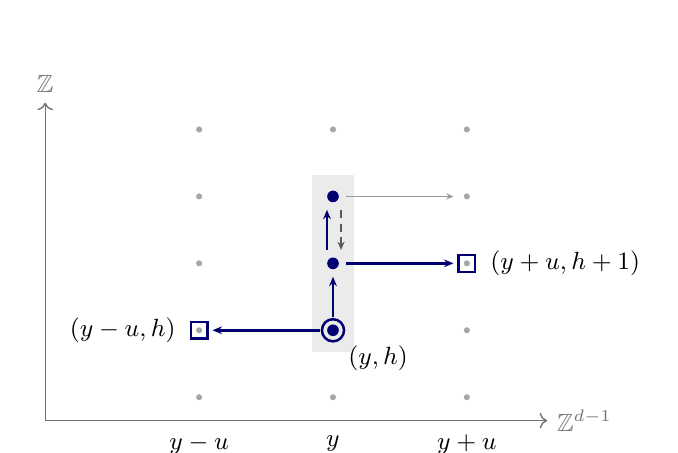
\begin{tikzpicture}[scale=0.85]
% Schematic of the column exploration from (y,h); horizontal axis: base Z^{j-1} (one direction shown), vertical axis: coordinate j.
\foreach \x in {-2,0,2} \foreach \z in {-1,...,3} \node[v] at (\x,\z) {};
\fill[explored] (-0.32,-0.32) rectangle (0.32,2.32);
\foreach \z in {0,1,2} \node[cv] at (0,\z) {};
\node[orig] at (0,0) {};
% root (y,h): chooses +e_j and -u
\draw[clus] (0,0.2) -- (0,0.8);
\draw[clus] (-0.2,0) -- (-1.8,0);
% (y,h+1): chooses +e_j and +u
\draw[clus] (-0.09,1.2) -- (-0.09,1.8);
\draw[clus] (0.2,1) -- (1.8,1);
% (y,h+2): chooses -e_j (ignored) and +u (already collected)
\draw[ign] (0.12,1.8) -- (0.12,1.2);
\draw[edge] (0.2,2) -- (1.8,2);
% entry points in neighbouring columns
\node[entry] at (-2,0) {};
\node[entry] at (2,1) {};
\node[left=5pt] at (-2,0) {\small $(y-u,h)$};
\node[right=5pt] at (2,1) {\small $(y+u,h+1)$};
\node[below right=2pt] at (0,0) {\small $(y,h)$};
% axis labels
\foreach \x/\l in {-2/{y-u},0/{y},2/{y+u}} \node at (\x,-1.7) {\small $\l$};
\draw[->,guide] (-4.3,-1.35) -- (3.2,-1.35) node[right] {\small $\Z^{d-1}$};
\draw[->,guide] (-4.3,-1.35) -- (-4.3,3.4) node[above] {\small $\Z$};

\end{tikzpicture}
\caption{Schematic column exploration from $(y,h)$; the horizontal axis represents $\Z^{d-1}$ by a single direction~$u$. The vertex $(y,h)$ chooses $+e_d$ and $-u$, the vertex $(y,h+1)$ chooses $+e_d$ and $+u$, and the vertex $(y,h+2)$ chooses $-e_d$, which plays no role (dashed), and $+u$. The explored set (shaded) is $E(y,h)=\{h,h+1,h+2\}$, the collected set is $M(y,h)=\{-u,+u\}$, and the squares mark the entry points $(y-u,h)$ and $(y+u,h+1)$ from which the neighbouring columns are explored.}
\label{fig:column}
\end{figure}

\begin{proposition}[Column projection]\label{prop:projection}
For every $d\ge3$ and every local law $\mu$ on the subsets of $\cD_d$ we have $\theta_d(\mu)\ge\theta_{d-1}(\Phi_d(\mu))$.
\end{proposition}

\begin{proof}
Fix an enumeration of $\Z^{d-1}$. We run the following exploration, which maintains a set $D$ of discovered vertices of $\Z^{d-1}$ with heights $h(y)\in\Z$, $y\in D$, and a set $S\subseteq D$ of processed vertices. Initially $D=\{o\}$, $h(o)=0$ and $S=\emptyset$. In step $i\ge1$, if $D\setminus S$ is empty, the exploration stops. Otherwise let $y_i$ be the element of $D\setminus S$ with the smallest index, set $M_i\coloneqq M(y_i,h(y_i))$, add $y_i$ to $S$, and add every $y_i+u$ with $u\in M_i$ and $y_i+u\notin D$ to $D$, with height $h(y_i+u)\coloneqq\eta(y_i,h(y_i),u)$.

\emph{Step 1: Lifting.} We show that $(y,h(y))\in\cC(o)$ for every $y\in D$, by induction over the order of discovery. This holds for $y=o$. If $y_i+u$ is discovered in step $i$ and $z\coloneqq\eta(y_i,h(y_i),u)$, then $(y_i,h(y_i))\rightsquigarrow(y_i,z)$ along the explored interval, and $(y_i,z)$ has an edge to $(y_i+u,z)=(y_i+u,h(y_i+u))$. Since $y\mapsto(y,h(y))$ is injective, we obtain $\#\cC(o)\ge\#D$.

\emph{Step 2: Law of $D$.} Let $\cG_i\coloneqq\sigma\big(y_l,\,N_{(y_l,z)}\colon l\le i,\ z\in\Z\big)$ be the $\sigma$-algebra generated by the first $i$ processed vertices and their columns. Whether the exploration stops after step $i$, and otherwise $y_{i+1}$ and $h(y_{i+1})$, are $\cG_i$-measurable. More precisely, for fixed distinct $z_1,\dots,z_i,y\in\Z^{d-1}$, the event $\{y_1=z_1,\dots,y_i=z_i,\,y_{i+1}=y\}$ depends only on the columns above $z_1,\dots,z_i$, which are independent of the column $\{y\}\times\Z$. Hence, conditionally on $\cG_i$ and on $y_{i+1}=y$, the choices in $\{y\}\times\Z$ are i.i.d.\ with law~$\mu$, and $M_{i+1}$ has law $\Phi_d(\mu)$. By induction over $i$, the sequence $(y_i,M_i)_i$ has the same law as the sequence produced by the same rule from an i.i.d.\ family $(\xi_y)_{y\in\Z^{d-1}}$ with law $\Phi_d(\mu)$, where $\xi_{y_i}$ replaces $M_i$; the heights do not enter the evolution of $D$ and $S$. In the latter exploration, every discovered vertex is processed after finitely many steps, because only finitely many vertices precede it in the enumeration, and processing $y$ discovers all its out-neighbours $y+\xi_y$. Hence $D$ has the law of the out-cluster of the origin in the site-i.i.d.\ model on $\Z^{d-1}$ with local law $\Phi_d(\mu)$, and $\P(\#D=\infty)=\theta_{d-1}(\Phi_d(\mu))$. Together with Step~1 this proves the claim.
\end{proof}

\begin{corollary}\label{cor:iterate}
For every $d\ge3$ and every local law $\mu$ on the subsets of $\cD_d$ we have
\begin{equation*}
\theta_d(\mu)\ge\theta_2\big(\Phi_3\circ\dots\circ\Phi_d(\mu)\big)\,.
\end{equation*}
\end{corollary}

\begin{proof}
Apply \cref{prop:projection} successively to the site-i.i.d.\ models on $\Z^d,\Z^{d-1},\dots,\Z^3$ with local laws $\mu$, $\Phi_d(\mu)$, $\Phi_{d-1}\circ\Phi_d(\mu)$, and so on. Only the resulting chain of inequalities between percolation probabilities is used.
\end{proof}

\subsection{The avoidance recursion}\label{sec:recursion}

To evaluate the right-hand side of \cref{cor:iterate} we track a finite family of numbers. A law $\mu$ on the subsets of $\cD_d$ is \emph{exchangeable} if it is invariant under all permutations of $\cD_d$. Then $t_\ell\coloneqq\mu(N\cap A=\emptyset)$ depends only on $\ell=\#A$, and we call $t=(t_0,\dots,t_{2d})$ the \emph{avoidance vector} of~$\mu$; it determines $\mu$. For $m\in\N$ let
\begin{equation*}
\cV_m\coloneqq\big\{t\in[0,1]^{m+1}\colon 1=t_0>t_1\ge t_2\ge\dots\ge t_m\big\}\,.
\end{equation*}
Avoidance vectors of exchangeable laws with $\mu(N=\emptyset)<1$ lie in $\cV_{2d}$. For $m\ge4$ and $t\in\cV_m$ we set $F(t)_0\coloneqq1$ and, for $1\le\ell\le m-2$,
\begin{equation}\label{eq:F}
\psi_\ell\coloneqq\frac{t_{\ell+1}}{1-t_\ell+t_{\ell+1}}\,,\qquad F(t)_\ell\coloneqq(1-\psi_\ell)^2\,t_{\ell+2}+2\psi_\ell(1-\psi_\ell)\,t_{\ell+1}+\psi_\ell^2\,t_\ell\,.
\end{equation}
The denominator is at least $1-t_\ell\ge1-t_1>0$.

\begin{lemma}[Monotonicity]\label{lem:monotone}
Let $m\ge4$. The map $F$ sends $\cV_m$ to $\cV_{m-2}$, and $t_{\ell+2}\le F(t)_\ell\le t_\ell$ for $1\le\ell\le m-2$. Moreover, $F$ is non-decreasing: if $t,t'\in\cV_m$ with $t\le t'$ componentwise, then $F(t)\le F(t')$.
\end{lemma}

\begin{proof}
On the set $\mathcal T\coloneqq\{(r_0,r_1,r_2)\colon1>r_0\ge r_1\ge r_2\ge0\}$ of ordered triples let $g(r_0,r_1)\coloneqq r_1/(1-r_0+r_1)$ and $H(r_0,r_1,r_2)\coloneqq(1-g)^2r_2+2g(1-g)r_1+g^2r_0$ with $g=g(r_0,r_1)$, so that $F(t)_\ell=H(t_\ell,t_{\ell+1},t_{\ell+2})$ for $\ell\ge1$; these triples lie in $\mathcal T$ because $t_\ell\le t_1<1$. The three weights in $H$ are non-negative and sum to one, which gives $r_2\le H\le r_0$. The function $g$ is non-decreasing in $r_0$ and in $r_1$, and
\begin{equation*}
\frac{\partial H}{\partial g}=2(1-g)(r_1-r_2)+2g(r_0-r_1)\ge0\,.
\end{equation*}
With the non-negative weights, all partial derivatives of $H$ are therefore non-negative on $\mathcal T$. If $(r_0,r_1,r_2)\le(r_0',r_1',r_2')$ both lie in $\mathcal T$, then raising first $r_0$ to $r_0'$, then $r_1$ to $r_1'$, and then $r_2$ to $r_2'$ keeps the triple in $\mathcal T$, so $H(r_0,r_1,r_2)\le H(r_0',r_1',r_2')$. This proves that $F$ is non-decreasing. Applied to the triples $(t_{\ell+1},t_{\ell+2},t_{\ell+3})\le(t_\ell,t_{\ell+1},t_{\ell+2})$ it gives $F(t)_{\ell+1}\le F(t)_\ell$ for $1\le\ell\le m-3$, and $F(t)_1\le t_1<1$ shows $F(t)\in\cV_{m-2}$.
\end{proof}

\begin{lemma}[Avoidance recursion]\label{lem:recursion}
Let $d\ge3$ and let $\mu$ be an exchangeable law on the subsets of $\cD_d$ with avoidance vector $t\in\cV_{2d}$. Then $\Phi_d(\mu)$ is exchangeable with avoidance vector $F(t)\in\cV_{2d-2}$.
\end{lemma}

\begin{proof}
The exploration in \cref{def:column} treats all horizontal directions alike, so $\Phi_d(\mu)$ is exchangeable. Fix $A\subseteq\cD_{d-1}$ with $\#A=\ell$, where $1\le\ell\le2d-2$, and consider the column exploration from $(o,0)$. Let $\varrho$ be the probability that no vertex $(o,z)$ with $z\ge1$ in $E(o,0)$ chooses a direction in $A$, given that $1\in E(o,0)$. The choices in $\{o\}\times\{1,2,\dots\}$ are independent of the choice of the root, so $\varrho$ does not depend on it. The vertex $(o,1)$ avoids $A\cup\{e_d\}$ with probability $t_{\ell+1}$, and then the exploration stops above. It avoids $A$ and chooses $e_d$ with probability $t_\ell-t_{\ell+1}$, and then the exploration continues from $(o,2)$ with fresh choices and the same law. Its choice of $-e_d$ plays no role. Hence $\varrho=t_{\ell+1}+(t_\ell-t_{\ell+1})\varrho$. Since $t_\ell-t_{\ell+1}\le t_1<1$, this equation has the unique solution $\varrho=\psi_\ell$. By symmetry, the same holds below the root.

At the root, exchangeability and inclusion--exclusion show that the probabilities to avoid $A$ and to choose neither, exactly one, or both of $\pm e_d$ are
\begin{equation*}
t_{\ell+2}\,,\qquad 2(t_{\ell+1}-t_{\ell+2})\,,\qquad t_\ell-2t_{\ell+1}+t_{\ell+2}\,.
\end{equation*}
Given the choice of the root, the parts above and below are independent. Therefore
\begin{equation*}
\Phi_d(\mu)(N\cap A=\emptyset)=t_{\ell+2}+2(t_{\ell+1}-t_{\ell+2})\,\psi_\ell+(t_\ell-2t_{\ell+1}+t_{\ell+2})\,\psi_\ell^2=F(t)_\ell\,.
\end{equation*}
For $\ell=0$ both sides equal one, and $F(t)\in\cV_{2d-2}$ by \cref{lem:monotone}.
\end{proof}

\cref{lem:monotone} is a statement about real vectors. In particular, rounding the entries upwards after an application of $F$, in a way that keeps them ordered, produces upper bounds for the exact avoidance vectors; we use this in \cref{sec:proof-bounds}.

\subsection{Comparison of consecutive dimensions}\label{sec:closure}

For $d\ge2$ let $\tau^{(d)}\in\cV_{2d}$ be the avoidance vector of $\mu_{d,2}$, that is,
\begin{equation*}
\tau^{(d)}_\ell=\frac{(2d-\ell)(2d-\ell-1)}{2d(2d-1)}\,,\qquad0\le\ell\le2d\,.
\end{equation*}
By \cref{lem:recursion}, the law $\nu_d\coloneqq\Phi_3\circ\dots\circ\Phi_d(\mu_{d,2})$ on the subsets of $\cD_2$ is exchangeable with avoidance vector $t^{(d)}\coloneqq F^{\circ(d-2)}(\tau^{(d)})\in\cV_4$. We now compare the recursions started in dimensions $d+1$ and $d$. One projection step from $\Z^{d+1}$ makes every set of size $\ell\le2d-2$ easier to hit than the $2$-neighbour graph on $\Z^d$ does.

\begin{lemma}[Consecutive dimensions]\label{lem:consecutive}
For all $d\ge2$ and $0\le\ell\le2d-2$ we have $F(\tau^{(d+1)})_\ell\le\tau^{(d)}_\ell$.
\end{lemma}

\begin{proof}
Let $m\coloneqq2d+2$ and $a\coloneqq m-\ell\in\{4,\dots,m\}$. Then $\tau^{(d+1)}_{\ell+i}=(a-i)(a-i-1)/(m(m-1))$ for $i\in\{0,1,2\}$, $\tau^{(d)}_\ell=(a-2)(a-3)/((m-2)(m-3))$, and
\begin{equation*}
1-\tau^{(d+1)}_\ell+\tau^{(d+1)}_{\ell+1}=\frac{m^2-m-2a+2}{m(m-1)}\,.
\end{equation*}
For $\ell=0$ both sides of the claim equal one, so let $\ell\ge1$, that is, $4\le a\le m-1$. Inserting these expressions into \cref{eq:F} and simplifying the rational function gives
\begin{equation}\label{eq:identity}
\tau^{(d)}_\ell-F(\tau^{(d+1)})_\ell=\frac{2(a-2)(a-m)\,W(a,m)}{m(m-1)(m-2)(m-3)\,(m^2-m-2a+2)^2}\,,
\end{equation}
where
\begin{equation*}
W(a,m)\coloneqq(3m^2-7m+6)\,a^2-(2m^4-7m^3+21m^2-26m+12)\,a+6m^4-17m^3+24m^2-19m+6\,.
\end{equation*}
The identity \cref{eq:identity} is an exact computation with rational functions, which we verified with a computer algebra system. For $4\le a\le m-1$ we have $(a-2)(a-m)<0$, and the denominator is positive because $m\ge6$ and $2a\le2m<m^2-m+2$. It thus remains to show $W(a,m)<0$ for $4\le a\le m-1$. Since $3m^2-7m+6>0$, the map $a\mapsto W(a,m)$ is convex, and it suffices to check the endpoints, where
\begin{equation*}
W(4,m)=-2m^4+11m^3-12m^2-27m+54\,,\qquad W(m-1,m)=-2(m-1)^2\,(m^3-7m^2+14m-12)\,.
\end{equation*}
The first expression is negative for $m\ge6$, since $m^3(11-2m)<0$ and $-12m^2-27m+54<0$. The cubic $m^3-7m^2+14m-12$ has the value $36$ at $m=6$ and the derivative $3m^2-14m+14>0$ for $m\ge4$, so $W(m-1,m)<0$ for $m\ge6$. Since $m=2d+2\ge6$, the claim follows.
\end{proof}

The set size $\ell=2d-1$ is not covered, and it cannot be: $\tau^{(d)}_{2d-1}=0$, whereas $F(\tau^{(d+1)})_{2d-1}>0$ because the projected out-set has size one with positive probability. We absorb the two largest entries by a closure. For $m\ge4$ and $t\in\cV_m$ let $Ct\in\cV_m$ be given by $(Ct)_\ell\coloneqq t_\ell$ for $\ell\le m-2$ and $(Ct)_{m-1}=(Ct)_m\coloneqq t_{m-2}$. Then $t\le Ct$, and $C$ is non-decreasing. With $G\coloneqq C\circ F$ we define
\begin{equation*}
\omega^{(d)}\coloneqq G^{\circ(d-2)}\big(C\tau^{(d)}\big)\in\cV_4\,,\qquad d\ge2\,.
\end{equation*}

\begin{lemma}[The closed recursion improves with the dimension]\label{lem:omega}
For all $d\ge3$ we have $t^{(d)}\le\omega^{(d)}$ and $\omega^{(d+1)}\le\omega^{(d)}$.
\end{lemma}

\begin{proof}
The first inequality follows from $t\le Ct$ and the monotonicity of $F$ and $C$ (\cref{lem:monotone}). For the second, the entry $F(t)_\ell$ involves only $t_\ell,t_{\ell+1},t_{\ell+2}$, and $C$ changes only the entries with index $2d+1$ and $2d+2$ of a vector in $\cV_{2d+2}$. Hence $F(C\tau^{(d+1)})_\ell=F(\tau^{(d+1)})_\ell\le\tau^{(d)}_\ell$ for $\ell\le2d-2$ by \cref{lem:consecutive}. Since $C$ on $\cV_{2d}$ only reads the entries with index at most $2d-2$, we obtain $G(C\tau^{(d+1)})\le C\tau^{(d)}$, and applying the non-decreasing map $G^{\circ(d-2)}$ yields $\omega^{(d+1)}\le\omega^{(d)}$.
\end{proof}

\subsection{Proof of the main results}\label{sec:proof-main}

It remains to start the comparison in a fixed dimension. The closure of \cref{sec:closure} costs too much in $d\le5$, where we use the exact vectors instead.

\begin{lemma}[Small dimensions]\label{lem:numbers}
Let $p=13/25$, so that $(1-p)^\ell$ equals $0.48$, $0.2304$, $0.110592$ and $0.05308416$ for $\ell=1,\dots,4$. Then $t^{(3)}$, $t^{(4)}$, $t^{(5)}$ and $\omega^{(6)}$ satisfy $t_\ell\le(1-p)^\ell$ for $\ell=1,\dots,4$. More precisely,
\begin{equation*}
t^{(3)}=\Big(1,\ \frac{53}{121},\ \frac{11}{80},\ \frac{9}{845},\ 0\Big)\,,
\end{equation*}
and, with all entries rounded upwards in the last digit,
\begin{align*}
t^{(4)}&\le(1,\ 0.35605,\ 0.09994,\ 0.00908,\ 0.00002)\,,\\
t^{(5)}&\le(1,\ 0.26695,\ 0.06770,\ 0.00613,\ 0.00002)\,,\\
\omega^{(6)}&\le(1,\ 0.18489,\ 0.04452,\ 0.04452,\ 0.04452)\,.
\end{align*}
\end{lemma}

\begin{proof}
For $d=3$ only one projection step occurs, and the recursion in the proof of \cref{lem:recursion} can be solved by hand. With $q\coloneqq\psi_\ell$ for $\tau^{(3)}$ one finds $q=6/11,\,1/4,\,1/13,\,0$ for $\ell=1,2,3,4$, and then
\begin{equation*}
t^{(3)}_\ell=\frac1{15}\Big(q^2+2(4-\ell)\,q+\binom{4-\ell}{2}\Big)\,,
\end{equation*}
which gives the stated values. The vectors $t^{(4)}$, $t^{(5)}$ and $\omega^{(6)}$ result from finitely many applications of \cref{eq:F} and of $C$, which we carried out in exact rational arithmetic.
\end{proof}

\begin{proof}[Proof of \cref{thm:main}]
Let $d\ge3$ and $p=13/25$. If $d\le5$, then $t^{(d)}_\ell\le(1-p)^\ell$ for $\ell=1,\dots,4$ by \cref{lem:numbers}. If $d\ge6$, then \cref{lem:omega} gives $t^{(d)}\le\omega^{(d)}\le\omega^{(6)}$, and the same bounds follow from \cref{lem:numbers}. In both cases \cref{lem:planar} applies to $\nu_d$, whose avoidance vector is $t^{(d)}$, and \cref{cor:iterate} yields
\begin{equation*}
\theta_d(2)=\theta_d(\mu_{d,2})\ge\theta_2(\nu_d)\ge\theta^\bond_2(13/25)>0\,.\qedhere
\end{equation*}
\end{proof}

\begin{proof}[Proof of \cref{cor:classification}]
For $k=1$ neither graph percolates \cite[Propositions~2.1 and~2.5]{JKLT25}. Choosing a uniform $(k+1)$-subset and deleting a uniformly chosen element produces a uniform $k$-subset, which couples the $k$- and the $(k+1)$-neighbour graphs monotonically. Hence it suffices to show that the directed $2$-neighbour graph percolates, because the undirected graph contains it. For $d=1$ every vertex chooses both neighbours, for $d=2$ we use \cite[Theorem~2.3]{CHJK26}, and for $d\ge3$ \cref{thm:main}.
\end{proof}

\subsection{Proof of the bounds on the critical mean out-degree}\label{sec:proof-bounds}

The local law $Q_{d,\beta}$ is exchangeable with avoidance vector
\begin{equation*}
\tau^{(d)}_\ell(\beta)=(2-\beta)\,\frac{2d-\ell}{2d}+(\beta-1)\,\frac{(2d-\ell)(2d-\ell-1)}{2d(2d-1)}\,,\qquad0\le\ell\le2d\,.
\end{equation*}
For each pair $(d,\bar\beta_d)$ in \cref{tab:bounds} we apply $F$ exactly $d-2$ times to $\tau^{(d)}(\bar\beta_d)$ in rational arithmetic and round every entry upwards to the grid $2^{-120}\Z$ after each step; rounding upwards keeps the vectors ordered. By \cref{lem:recursion,lem:monotone}, the result bounds the avoidance vector of $\Phi_3\circ\dots\circ\Phi_d(Q_{d,\bar\beta_d})$ from above. In every case its entries satisfy $t_\ell<2^{-\ell}$ for $\ell=1,\dots,4$, so \cref{lem:planar} applies with some $p>1/2$, and \cref{cor:iterate} gives $\theta_d(Q_{d,\bar\beta_d})>0$. By monotonicity in $\beta$ \cite[Lemma~2.1]{CHJK26}, this proves $\beta_{\mathrm c}(d)\le\bar\beta_d$.

\section*{Code and data}
The scripts for the exact computations in \cref{lem:consecutive,lem:numbers}, for the bounds and simulations in \cref{tab:bounds}, for the numerical observations in \cref{sec:discussion} and for \cref{fig:model} are available from the authors.

\section*{Disclosure of the use of AI}
The column projection, the avoidance recursion, \cref{lem:consecutive} and the closure argument were found with substantial assistance of the AI system Claude (Anthropic). Claude also wrote the computer code for the exact and rigorous numerical computations and the simulations, and drafted this manuscript and its figures. The authors have checked all mathematical arguments and computations and take full responsibility for the content of this paper.

\bibliographystyle{amsalpha}
\bibliography{refs}

\end{document}
